%%%%%%%%%%%%%%%%%%%%%%%%%%%%%%%%%%%%%%%%%
% Beamer Presentation
% LaTeX Template
% Version 1.0 (10/11/12)
%
% This template has been downloaded from:
% http://www.LaTeXTemplates.com
%
% License:
% CC BY-NC-SA 3.0 (http://creativecommons.org/licenses/by-nc-sa/3.0/)
%
%%%%%%%%%%%%%%%%%%%%%%%%%%%%%%%%%%%%%%%%%

%----------------------------------------------------------------------------------------
%	PACKAGES AND THEMES
%----------------------------------------------------------------------------------------

\documentclass{beamer}
\usepackage{xcolor}
\usepackage{lmodern}
\usepackage[ruled,vlined]{algorithm2e}
\usepackage{subcaption}

\mode<presentation> {

% The Beamer class comes with a number of default slide themes
% which change the colors and layouts of slides. Below this is a list
% of all the themes, uncomment each in turn to see what they look like.

%\usetheme{default}
%\usetheme{AnnArbor}
%\usetheme{Antibes}
%\usetheme{Bergen}
%\usetheme{Berkeley}
%\usetheme{Berlin}
%\usetheme{Boadilla}
\usetheme{CambridgeUS}
%\usetheme{Copenhagen}
%\usetheme{Darmstadt}
%\usetheme{Dresden}
%\usetheme{Frankfurt}
%\usetheme{Goettingen}
%\usetheme{Hannover}
%\usetheme{Ilmenau}
%\usetheme{JuanLesPins}
%\usetheme{Luebeck}
%\usetheme{Madrid}
%\usetheme{Malmoe}
%\usetheme{Marburg}
%\usetheme{Montpellier}
%\usetheme{PaloAlto}
% \usetheme{Pittsburgh}
%\usetheme{Rochester}
%\usetheme{Singapore}
%\usetheme{Szeged}
%\usetheme{Warsaw}

% As well as themes, the Beamer class has a number of color themes
% for any slide theme. Uncomment each of these in turn to see how it
% changes the colors of your current slide theme.

%\usecolortheme{albatross}
%\usecolortheme{beaver}
%\usecolortheme{beetle}
%\usecolortheme{crane}
\usecolortheme{dolphin}
%\usecolortheme{dove}
%\usecolortheme{fly}
%\usecolortheme{lily}
% \usecolortheme{orchid}
%\usecolortheme{rose}
%\usecolortheme{seagull}
%\usecolortheme{seahorse}
%\usecolortheme{whale}
%\usecolortheme{wolverine}

%\setbeamertemplate{footline} % To remove the footer line in all slides uncomment this line
%\setbeamertemplate{footline}[page number] % To replace the footer line in all slides with a simple slide count uncomment this line

%\setbeamertemplate{navigation symbols}{} % To remove the navigation symbols from the bottom of all slides uncomment this line
\setbeamercovered{transparent}
}

\usepackage{graphicx} % Allows including images
\usepackage{booktabs} % Allows the use of \toprule, \midrule and \bottomrule in tables

%----------------------------------------------------------------------------------------
%	TITLE PAGE
%----------------------------------------------------------------------------------------

\title[WPSS implemented over WebRTC]{The Wormhole Peer Sampling Service implemented over WebRTC} % The short title appears at the bottom of every slide, the full title is only on the title page

\author{Davide Spadini} % Your name
\institute[Unitn] % Your institution as it will appear on the bottom of every slide, may be shorthand to save space
{
University of Trento \\ % Your institution for the title page
\medskip
\textit{davide.spadini@unitn.it} % Your email address
}
\date{\today} % Date, can be changed to a custom date

\begin{document}

\begin{frame}
\titlepage % Print the title page as the first slide
\end{frame}

\begin{frame}
\frametitle{Overview} % Table of contents slide, comment this block out to remove it
\tableofcontents % Throughout your presentation, if you choose to use \section{} and \subsection{} commands, these will automatically be printed on this slide as an overview of your presentation
\end{frame}

%----------------------------------------------------------------------------------------
%	PRESENTATION SLIDES
%----------------------------------------------------------------------------------------

%-----------------------------------------------------------------------------------------------------------------------------
\section{Wormhole Peer Sampling Service} % Sections can be created in order to organize your presentation into discrete blocks, all sections and subsections are automatically printed in the table of contents as an overview of the talk
\begin{frame}[c]
\Huge{\centerline{Wormhole Peer Sampling Service}}

\end{frame}

%-----------------------------------------------------------------------------------------------------------------------------
\subsection{Introduction}

\begin{frame}
\frametitle{Introduction}
A peer sampling service (PSS) is a service that runs on all the nodes in a distributed system and provides them with a uniform random sample of live nodes from all nodes in the system, where the sample size is typically much smaller than the system size. 
\end{frame}


\begin{frame}
\frametitle{The idea}
\begin{columns}[t] % The "c" option specifies centered vertical alignment while the "t" option is used for top vertical alignment

\column{.5\textwidth} % Left column and width
\textbf{Past}
\begin{enumerate}
\item Relatively small size
\item (Almost) static network
\item Nodes have {\color{red}{full}} view of the network
\end{enumerate}

\column{.5\textwidth} % Right column and width
\textbf{Now}
\begin{enumerate}
\item Big size
\item Dynamic network
\item Nodes have {\color{red}{partial}} view of the network
\end{enumerate}
\end{columns}\end{frame}


\begin{frame}
\frametitle{Implementation}
A PSS can be implemented:
\begin{itemize}
	\item as a \textbf{centralized service}: expensive to run reliably
	\item using \textbf{gossip protocols}: the most widely adopted solution
	\item using \textbf{random walks}: suitable for stable networks
\end{itemize}
\end{frame}

\begin{frame}
\frametitle{The problems}
\begin{columns}[t] % The "c" option specifies centered vertical alignment while the "t" option is used for top vertical alignment

\column{.5\textwidth} % Left column and width
\textbf{First problem:}

\begin{itemize}
	\item Network Address Translation (NAT)
	\item Firewall
	\item Antivirus
	\item etc etc..
\end{itemize}

\pause
\textbf{Solution:}

Gossip-based NAT-aware Peer Sampling Service


\column{.5\textwidth} % Right column and width
\textbf{Second problem:}
\begin{itemize}
	\item Require peers to frequently establish network connections and exchange messages with nodes that support direct connectivity
	\item It is a complex and costly procedure!
\end{itemize}
\pause
\textbf{Solution:}

Wormhole Peer Sampling Service!

\end{columns}
\end{frame}

%-----------------------------------------------------------------------------------------------------------------------------
\subsection{WPSS}

\begin{frame}
\begin{itemize}
	\item Published in 2013
	\item It has the same levels of samples' freshness  of the other PSSes, while the connection establishment rate is decreased by one order of magnitude
	\pause
	\item \textbf{Main idea}: to divide the service into two layers
\end{itemize}
\end{frame}

\begin{frame}
\frametitle{Overlays}

\begin{figure}
\includegraphics[keepaspectratio=true, width=\textwidth]{images/overlay}
\end{figure}

\end{frame}

%-----------------------------------------------------------------------------------------------------------------------------
\subsection{WPSS: The algorithm}
% \renewcommand{\thealgocf}{}

\begin{frame}[fragile] % Need to use the fragile option when verbatim is used in the slide
\frametitle{The algorithm}

\begin{algorithm}[H]
  \SetKwProg{Upon}{upon}{ do}{end}
  \SetKwProg{Every}{every}{ do}{end}

  \Upon{wormholeFailure}{
  	$wormhole \leftarrow tracker.getNewWormhole()$\;
    $connect(wormhole)$\;
  }

  \Upon{baseOverlayFailure}{
  	$peer \leftarrow tracker.getNewPeer()$\;
  	$connect(peer)$
  }
 \caption{Wormhole peer sampling}
\end{algorithm}

\end{frame}

\begin{frame}[fragile] % Need to use the fragile option when verbatim is used in the slide
\frametitle{The algorithm}

\begin{algorithm}[H]
  \SetKwProg{Upon}{upon}{ do}{end}
  \SetKwProg{Every}{every}{ do}{end}

  \Every{$\Delta_{wh}$ = wormholeTimeout}{
    $disconnect(wormhole)$\;
  	$wormhole \leftarrow tracker.getNewWormhole()$\;
    $connect(wormhole)$\;
  }

  \Every{$\Delta$ = adTimeout}{
  	$ad \leftarrow createAd()$\;
  	$ad.hops \leftarrow 1$\;
  	$sendAdToWormhole(wormhole, ad)$\;
  }
  \caption{Wormhole peer sampling}
\end{algorithm}

\end{frame}
  
\begin{frame}
\frametitle{The algorithm}
    
\begin{algorithm}[H]
  \SetKwProg{Upon}{upon}{ do}{end}
  \SetKwProg{Every}{every}{ do}{end}

  \Upon{receivedAd(ad)}{
  	\If{ad.hop = getTTL() $\mid\mid$ acceptAd(ad)}{
  		view.addAd(ad)
  	}\Else{
  		$neighbour \leftarrow getMetropolisHastingsNeighbour()$\;
  		$ad.hop \leftarrow ad.hop + 1$\;
  		$sendAd(neighbour, ad)$\;
  	}
  }
  \caption{Wormhole peer sampling}
\end{algorithm}
\end{frame}



%-----------------------------------------------------------------------------------------------------------------------------
\section{WebRTC}

\begin{frame}[c]
\Huge{\centerline{WebRTC}}

\end{frame}


\begin{frame}\frametitle{Three main tasks}
\begin{itemize}
  \item Acquiring audio and video: getting access to the microphone or camera, getting a streaming of media for either of them
  \item Communicating audio and video: being able to connect to another WebRTC end-point through Internet, and send audio and video stream in real-time
  \item Communicating generic data: not only audio and video, but for any arbitrary application data
\end{itemize}    
\end{frame}

\begin{frame}\frametitle{Three JavaScript APIs}

\begin{itemize}
  \item\textbf{\textsf{MediaStream} (aka getUserMedia)}
  \item\textbf{\textsf{RTCPeerConnection}}
  \item\textbf{\textsf{RTCDataChannel}}
\end{itemize}
\end{frame}

%-----------------------------------------------------------------------------------------------------------------------------
\subsection{Signaling}

\begin{frame}\frametitle{Signaling}
    
Abstract Signaling
\begin{itemize}
  \item Need to exchange ``session description'' objects:
  \begin{itemize}
    \item What formats I support, what I want to send
    \item Network information for peer-to-peer setup
  \end{itemize}
  \item Can use any messaging mechanism
  \item Can use any messaging protocol
\end{itemize}
\end{frame}


\begin{frame}[c]\frametitle{Signaling}

\begin{figure}
\centering
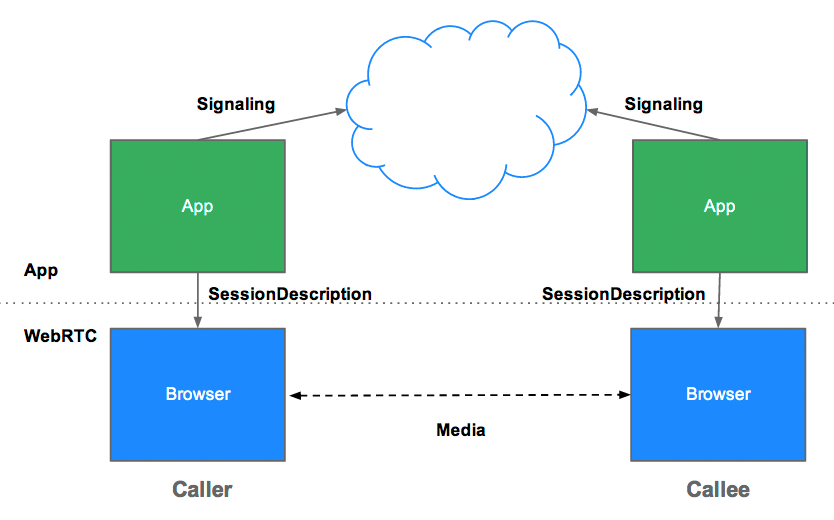
\includegraphics[width=0.9\textwidth]{images/jsep}
\end{figure}

\end{frame}

%-----------------------------------------------------------------------------------------------------------------------------
\subsection{STUN and TURN Servers}

\begin{frame}[t]\frametitle{STUN and TURN Servers}
\begin{figure}
\centering

\includegraphics[keepaspectratio=true, width=0.9\textwidth]{images/noSTUNorTURN}
\end{figure}
\end{frame}



\begin{frame}[t]\frametitle{STUN and TURN Servers}
\begin{figure}
\centering
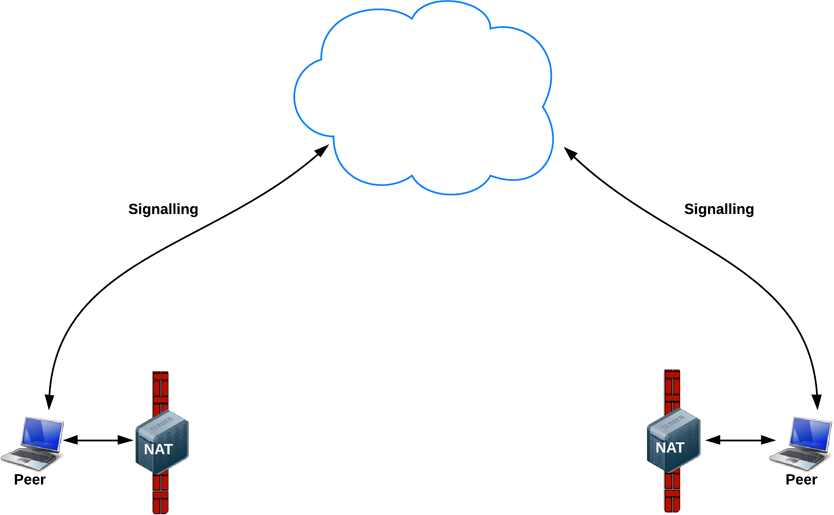
\includegraphics[keepaspectratio=true, width=0.9\textwidth]{images/firewall}
\end{figure}
\end{frame}

\begin{frame}[t]\frametitle{STUN and TURN Servers}
\begin{figure}
\centering
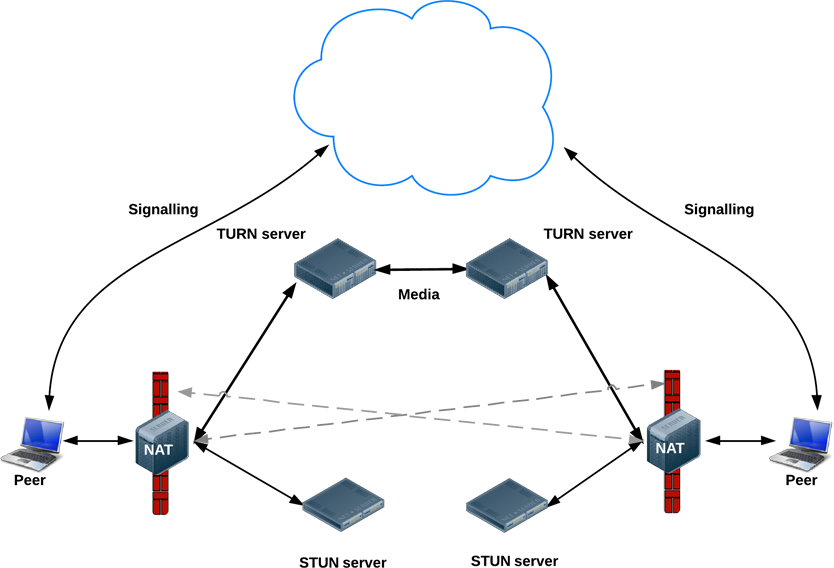
\includegraphics[keepaspectratio=true, width=0.9\textwidth]{images/turn}
\end{figure}
\end{frame}


%-----------------------------------------------------------------------------------------------------------------------------
\subsection{EasyRTC}

\begin{frame}\frametitle{Back to reality: EasyRTC Framework}
\begin{itemize}
  \item Establishing a connection between two peers in WebRTC is not so simple.
  \item With power comes complexity
  \item To hide that complexity, Priologic\footnote{A team of Canadian software developers. More information: \url{https://www.priologic.com}} has built the EasyRTC framework.
  \item Tracker
\end{itemize}
\end{frame}


%-----------------------------------------------------------------------------------------------------------------------------
\section{Evaluation}

\begin{frame}[c]
\Huge{\centerline{Evaluation}}

\end{frame}

\begin{frame}\frametitle{Environment}
Emulation environment:
\begin{itemize}
  \item $N = 1000$
  \item $View$ $Size = 50$
  \item $TTL = 100$
\end{itemize}
\end{frame}

%-----------------------------------------------------------------------------------------------------------------------------
\subsection{Freshness}

\begin{frame}
\frametitle{Average hop count}

\begin{figure}
\centering
\begin{subfigure}{.5\textwidth}
  \centering
  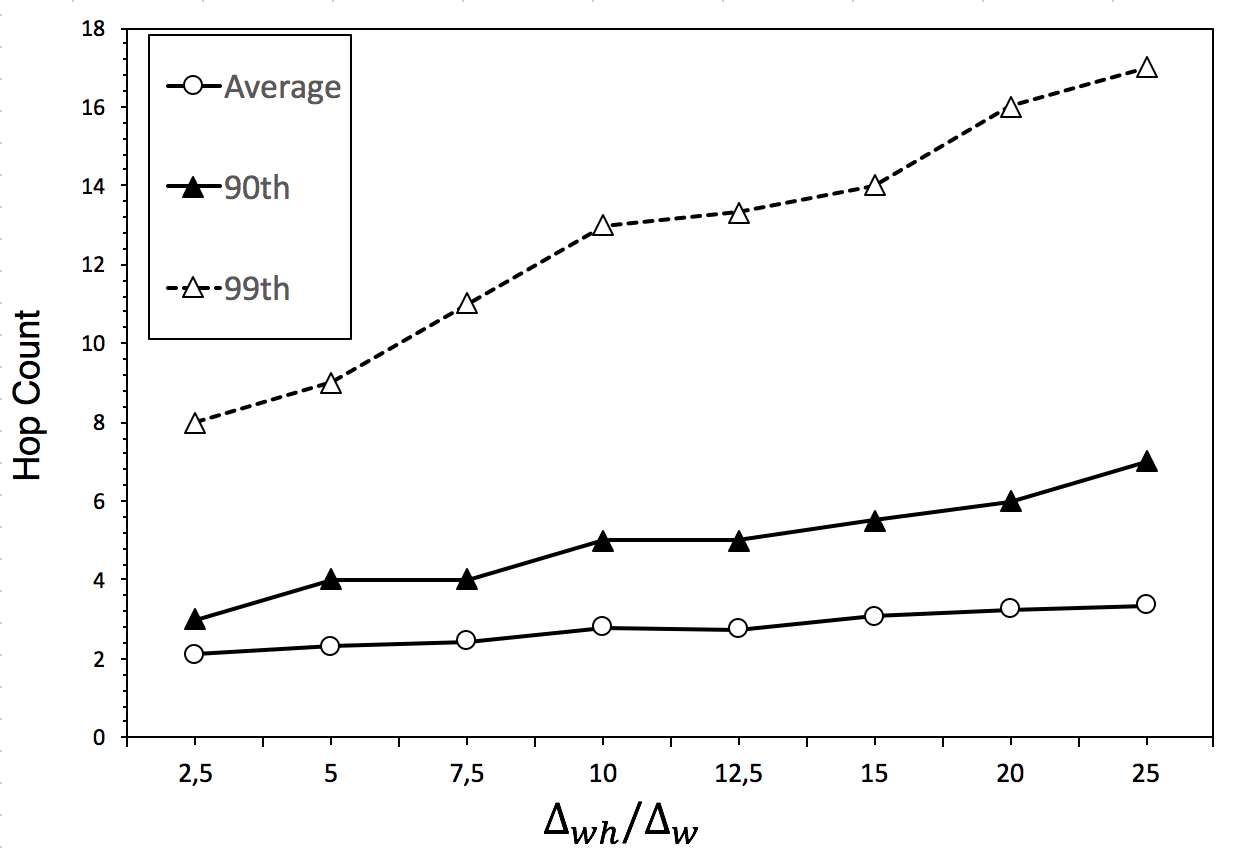
\includegraphics[keepaspectratio=true, width=1\linewidth]{images/average_hop_count}
  \caption{}
  \label{fig:my_average_hop_count}
\end{subfigure}%
\begin{subfigure}{.5\textwidth}
  \centering
  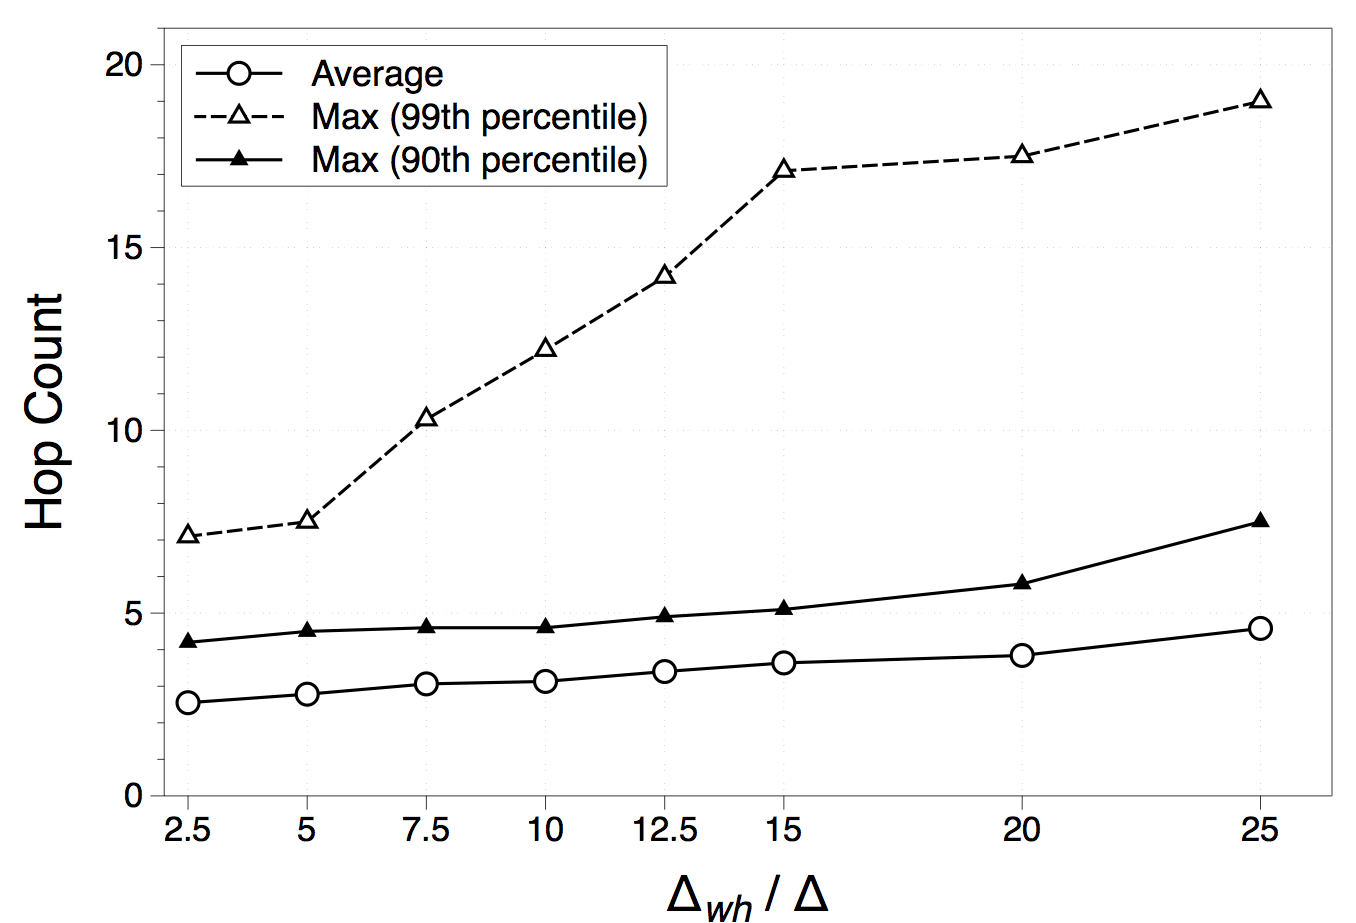
\includegraphics[keepaspectratio=true, width=1\linewidth]{images/paper_average_hop_count}
  \caption{}
  \label{fig:paper_average_hop_count}
\end{subfigure}
\caption{Measure of the average hop count, as well as the $90^{th}$ and $99^{th}$ percentile.~\ref{fig:my_average_hop_count} represents our result,~\ref{fig:paper_average_hop_count} is the test reported in the paper.}
\label{fig:freshness}
\end{figure}
\end{frame}

%-----------------------------------------------------------------------------------------------------------------------------
\subsection{Robustness}

\begin{frame}
\frametitle{Hop count in a flash crowd scenario}

\begin{figure}
\centering
\begin{subfigure}{.5\textwidth}
  \centering
  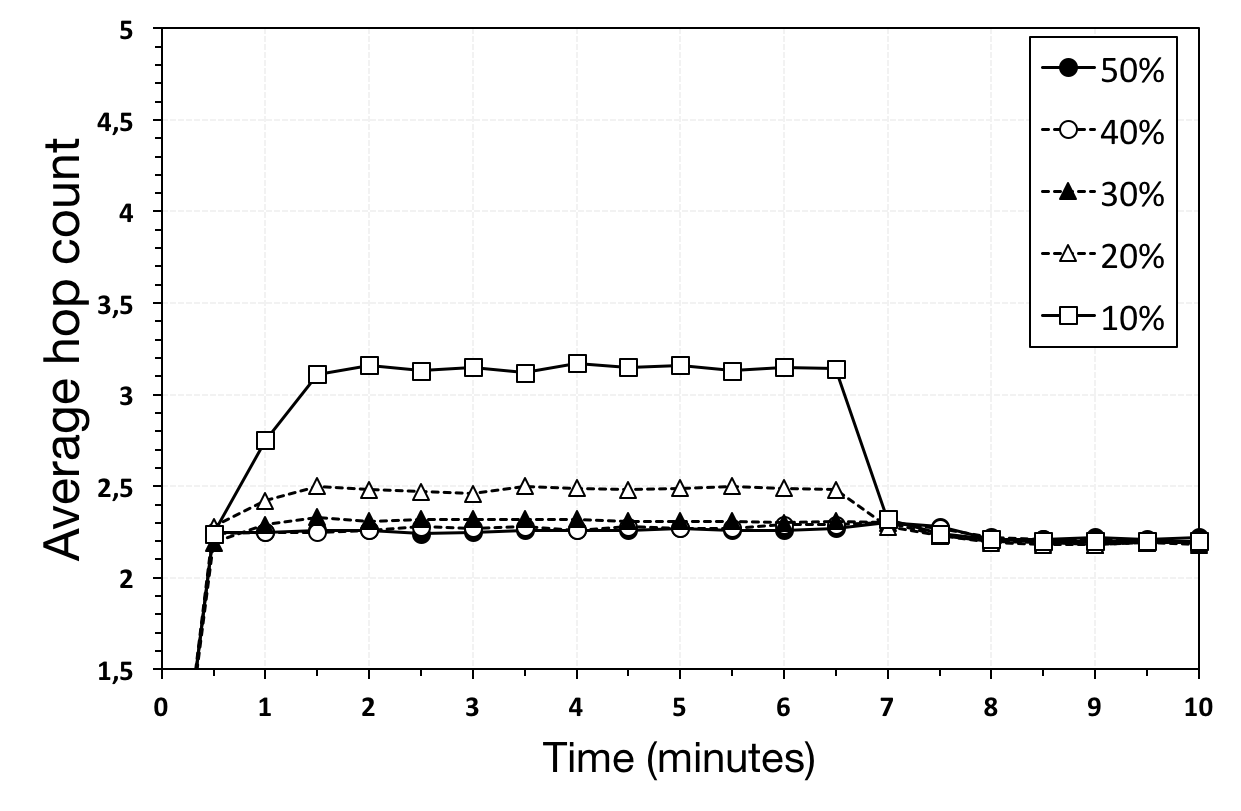
\includegraphics[keepaspectratio=true, width=1\linewidth]{images/average_hop_count_flash_crowd_1impl}
  \caption{}
  \label{fig:average_hop_count_flash_crowd_1impl}
\end{subfigure}%
\begin{subfigure}{.5\textwidth}
  \centering
  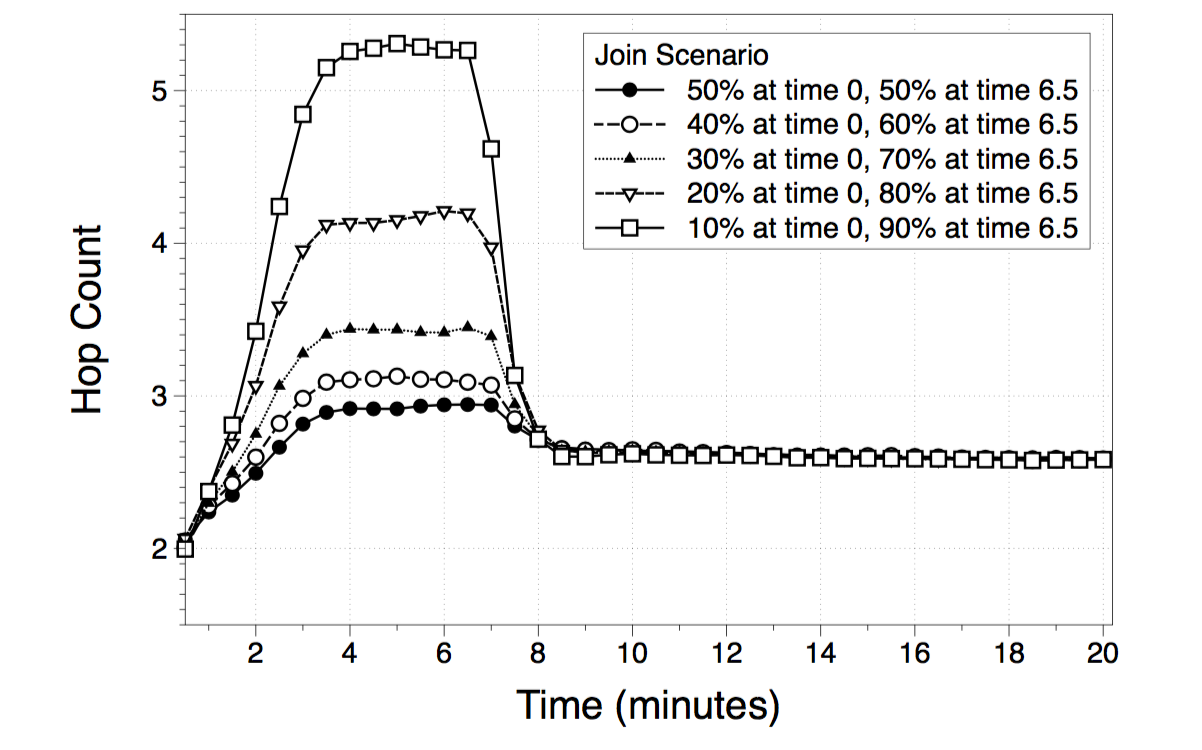
\includegraphics[keepaspectratio=true, width=1\linewidth]{images/paper_average_hop_count_flash_crowd}
  \caption{}
  \label{fig:paper_average_hop_count_flash_crowd}
\end{subfigure}
\caption{Average hop count in a flash crowd scenario.~\ref{fig:average_hop_count_flash_crowd_1impl} represents our result,~\ref{fig:paper_average_hop_count_flash_crowd} is the test reported in the paper.}
\label{fig:robustness_hop_count_flash_crowd}
\end{figure}

\end{frame}

\begin{frame}
\frametitle{Average in-degree}

\begin{figure}
\centering
\begin{subfigure}{.5\textwidth}
  \centering
  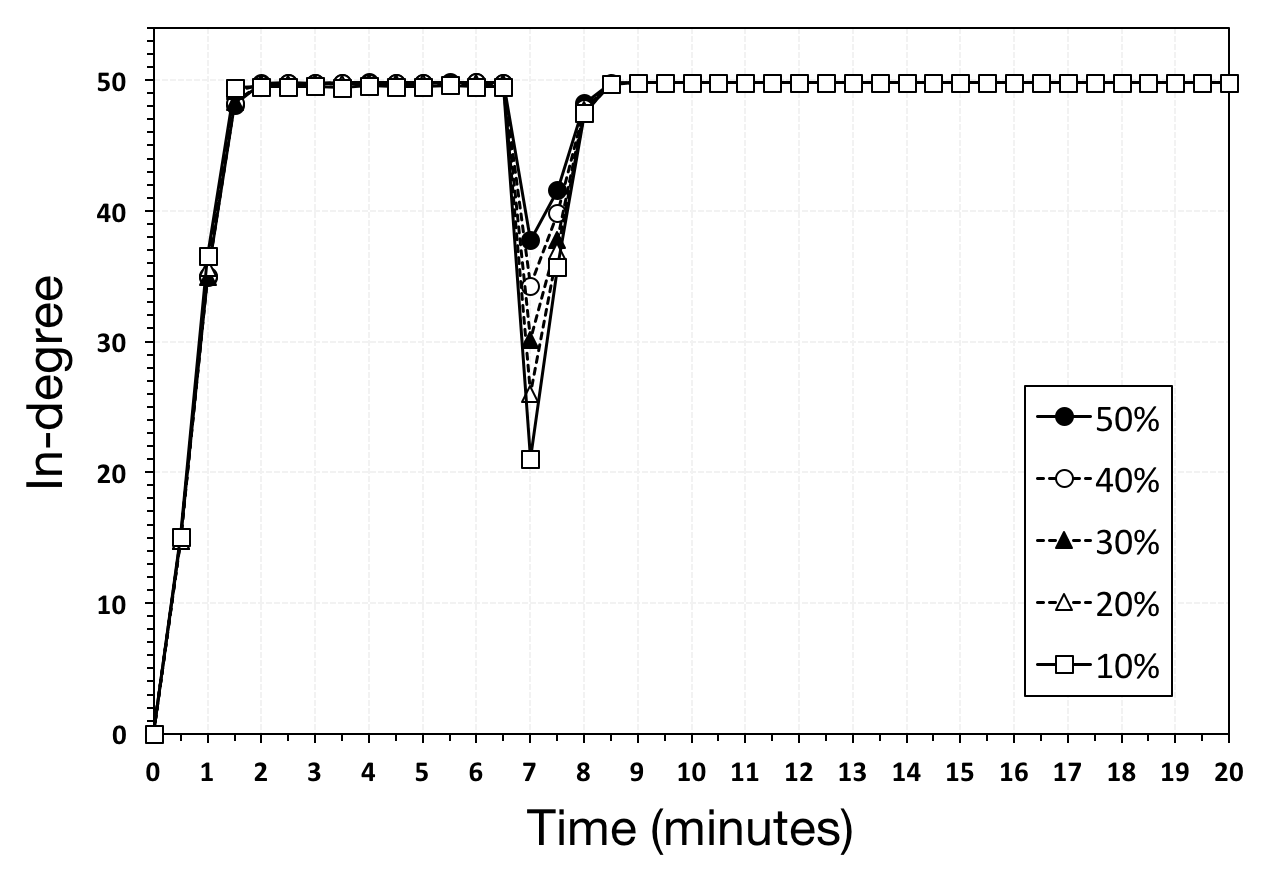
\includegraphics[keepaspectratio=true, width=1\linewidth]{images/average_indegree}
  \caption{}
  \label{fig:average_indegree}
\end{subfigure}%
\begin{subfigure}{.5\textwidth}
  \centering
  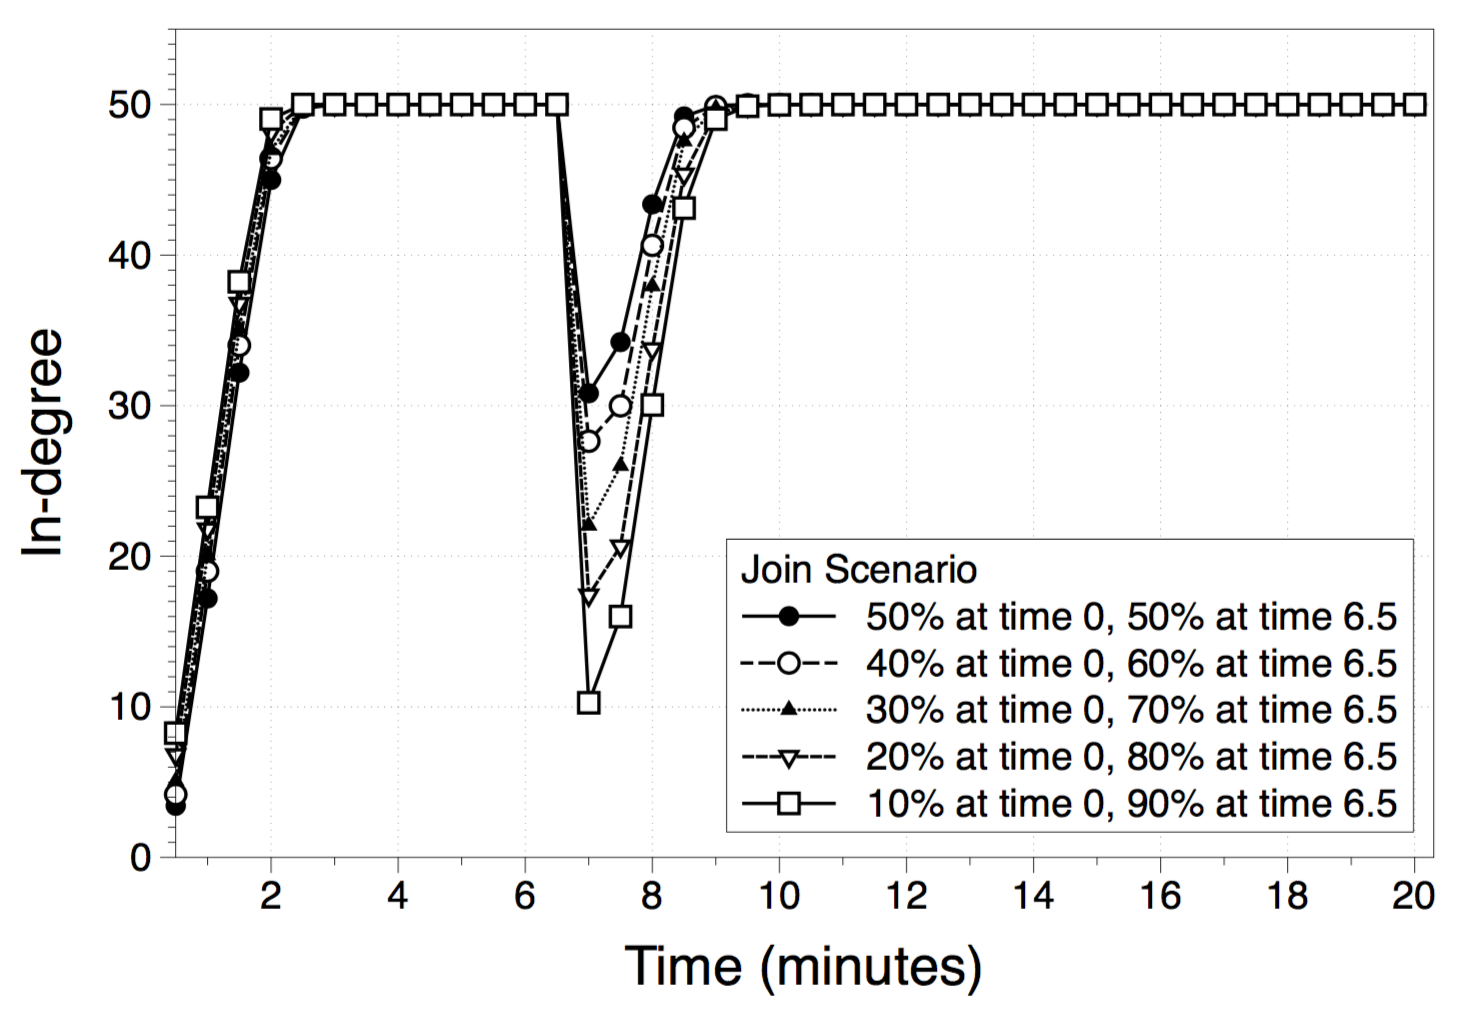
\includegraphics[keepaspectratio=true, width=1\linewidth]{images/paper_average_indegree}
  \caption{}
  \label{fig:paper_average_indegree}
\end{subfigure}
\caption{Average in-degree in a flash crowd scenario.~\ref{fig:average_indegree} represents our result,~\ref{fig:paper_average_indegree} is the test reported in the paper.}
\label{fig:robustness_indegree_flash_crowd}
\end{figure}

\end{frame}

\begin{frame}
\frametitle{Hop count in a massive failure scenario}

\begin{figure}
\centering
\begin{subfigure}{.5\textwidth}
  \centering
  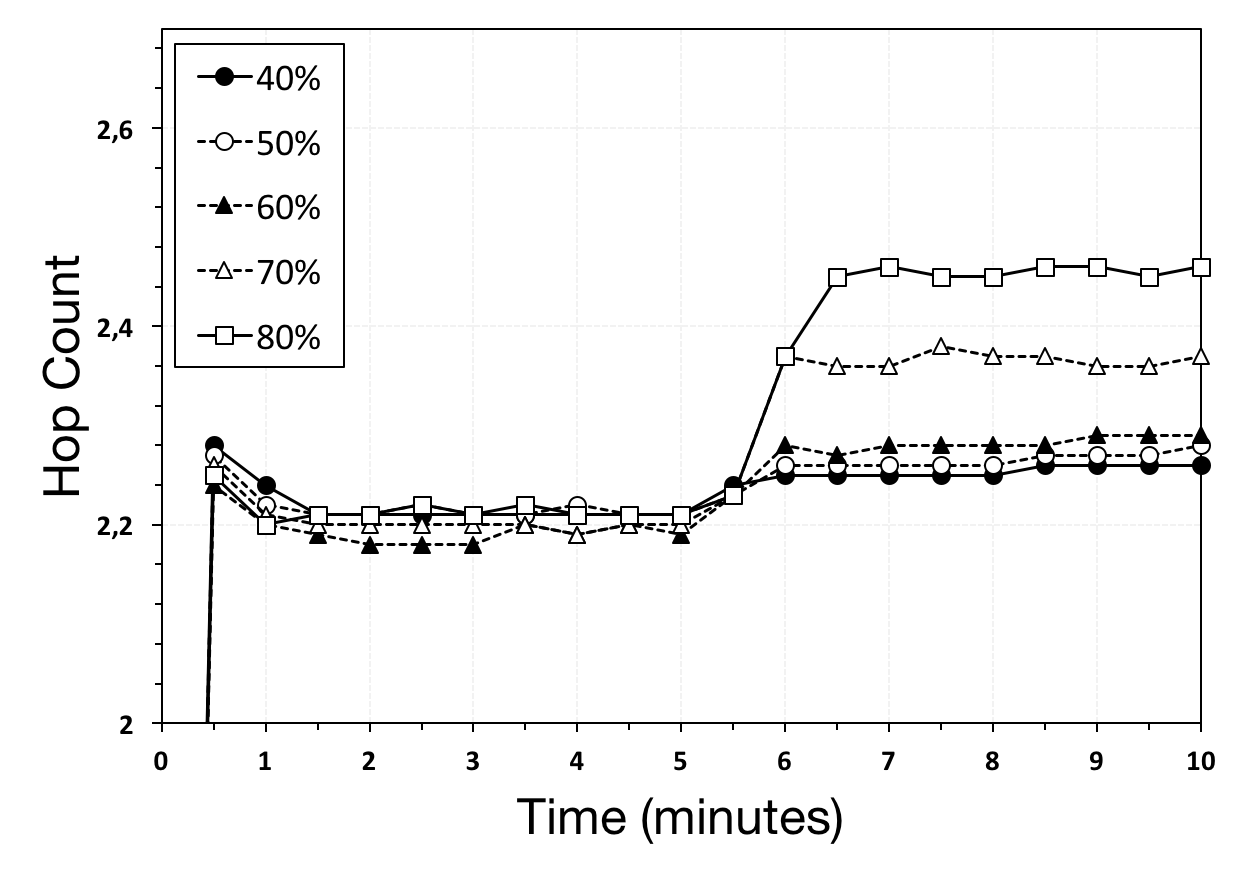
\includegraphics[keepaspectratio=true, width=1\linewidth]{images/average_hop_count_failures_1impl}
  \caption{}
  \label{fig:average_hop_count_failures_1impl}
\end{subfigure}%
\begin{subfigure}{.5\textwidth}
  \centering
  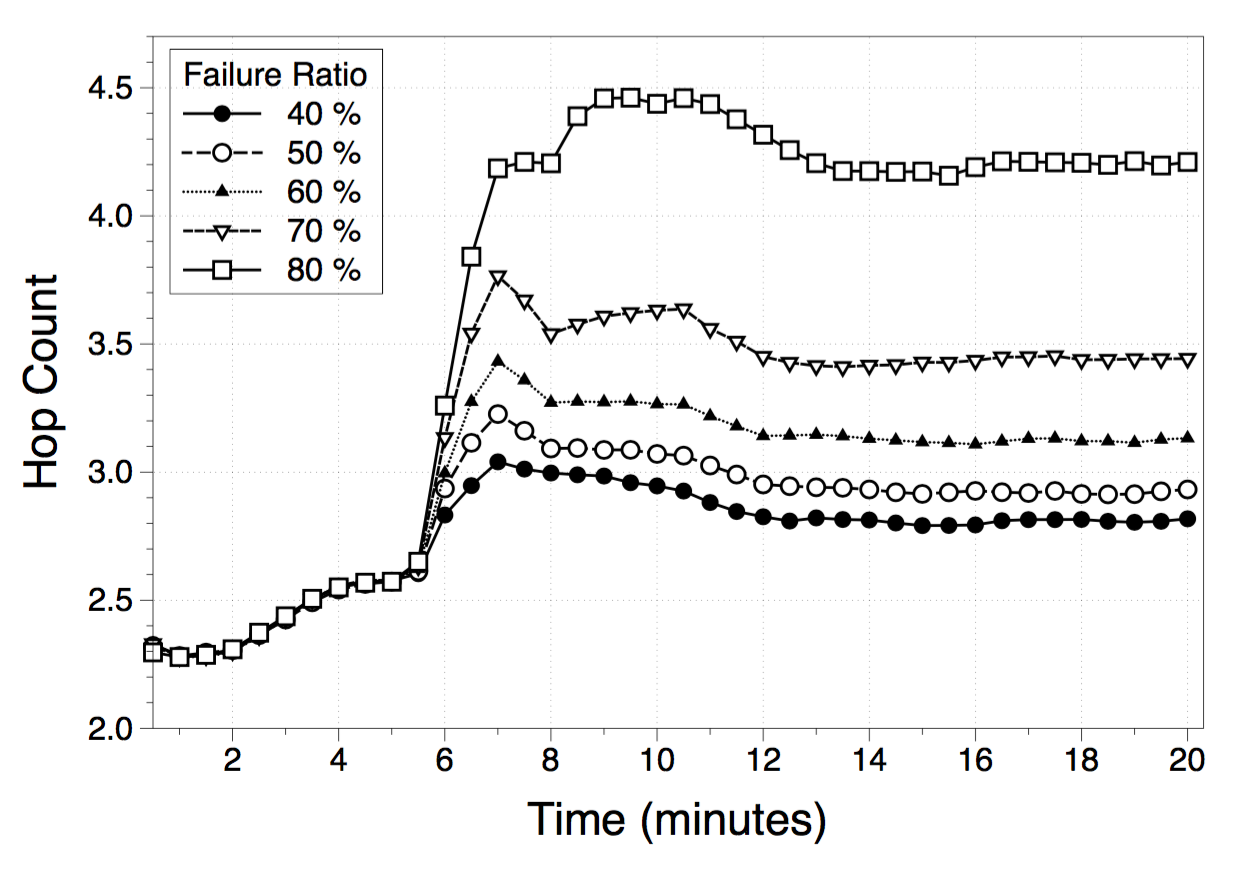
\includegraphics[keepaspectratio=true, width=1\linewidth]{images/paper_average_hop_count_failures}
  \caption{}
  \label{fig:paper_average_hop_count_failures}
\end{subfigure}
\caption{Average hop count in a flash crowd scenario.~\ref{fig:average_hop_count_failures_1impl} represents our result,~\ref{fig:paper_average_hop_count_failures} is the test reported in the paper.}
\label{fig:robustness_hop_count_failures}
\end{figure}

\end{frame}

\begin{frame}
\frametitle{Average number of dead links}
    
\begin{figure}
\centering
\begin{subfigure}{.5\textwidth}
  \centering
  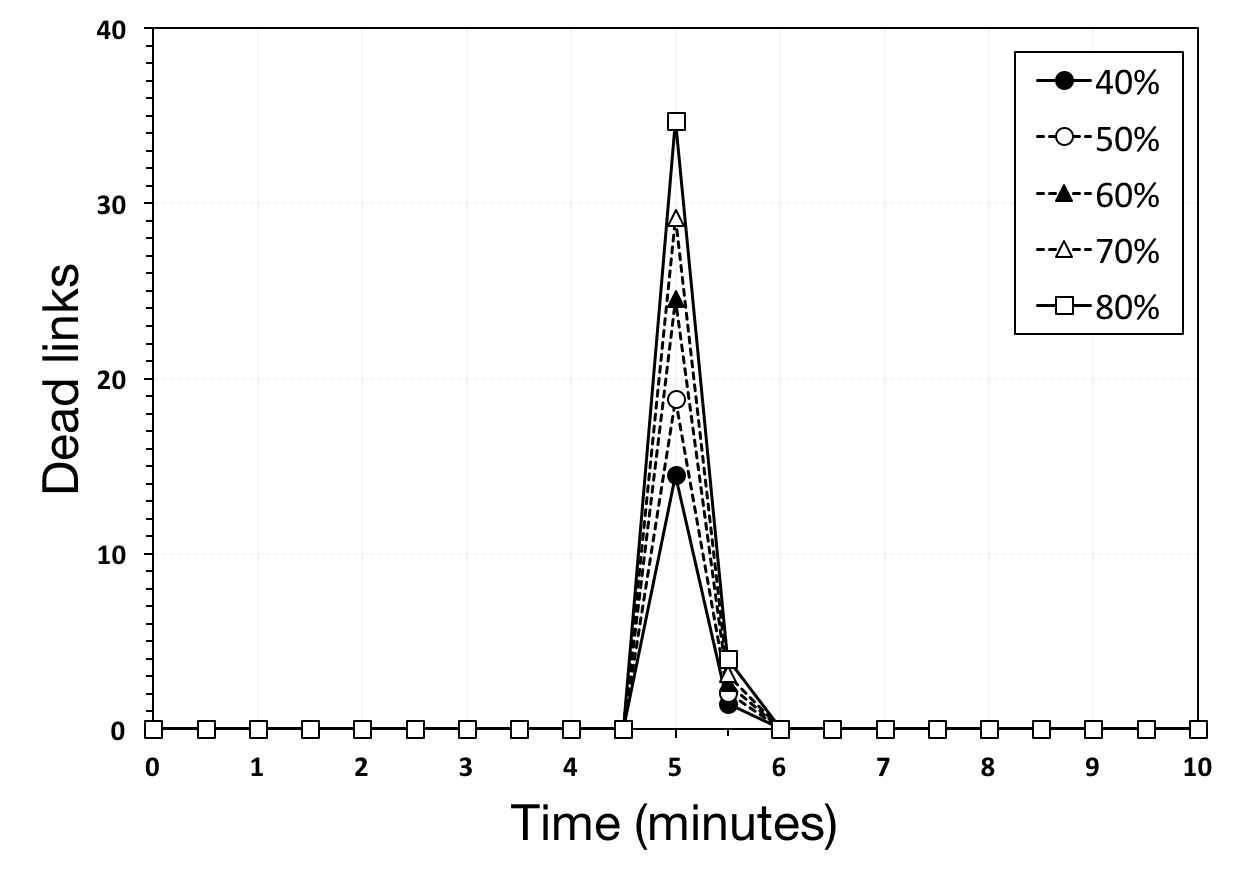
\includegraphics[keepaspectratio=true, width=1\linewidth]{images/average_dead_links}
  \caption{}
  \label{fig:average_dead_links}
\end{subfigure}%
\begin{subfigure}{.5\textwidth}
  \centering
  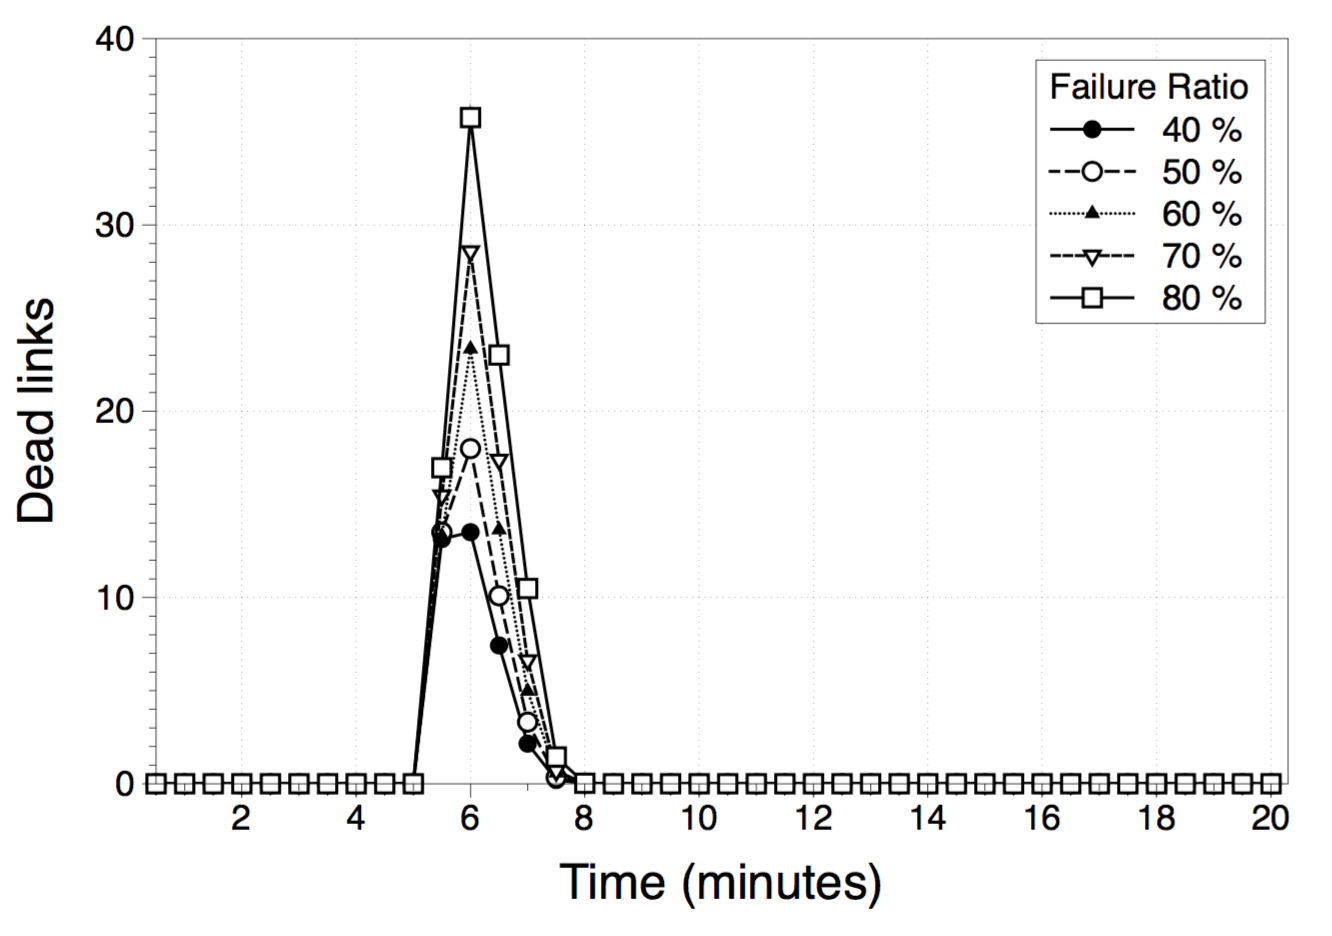
\includegraphics[keepaspectratio=true, width=1\linewidth]{images/paper_average_dead_links}
  \caption{}
  \label{fig:paper_average_dead_links}
\end{subfigure}
\caption{Average number of dead links in a flash crowd scenario.~\ref{fig:average_dead_links} represents our result,~\ref{fig:paper_average_dead_links} is the test reported in the paper.}
\label{fig:robustness_dead_links_failures}
\end{figure}

\end{frame}

%-----------------------------------------------------------------------------------------------------------------------------
\subsection{Churn}

\begin{frame}
\frametitle{Hop count with different levels of churn}
    
\begin{figure}
\centering
\begin{subfigure}{.5\textwidth}
  \centering
  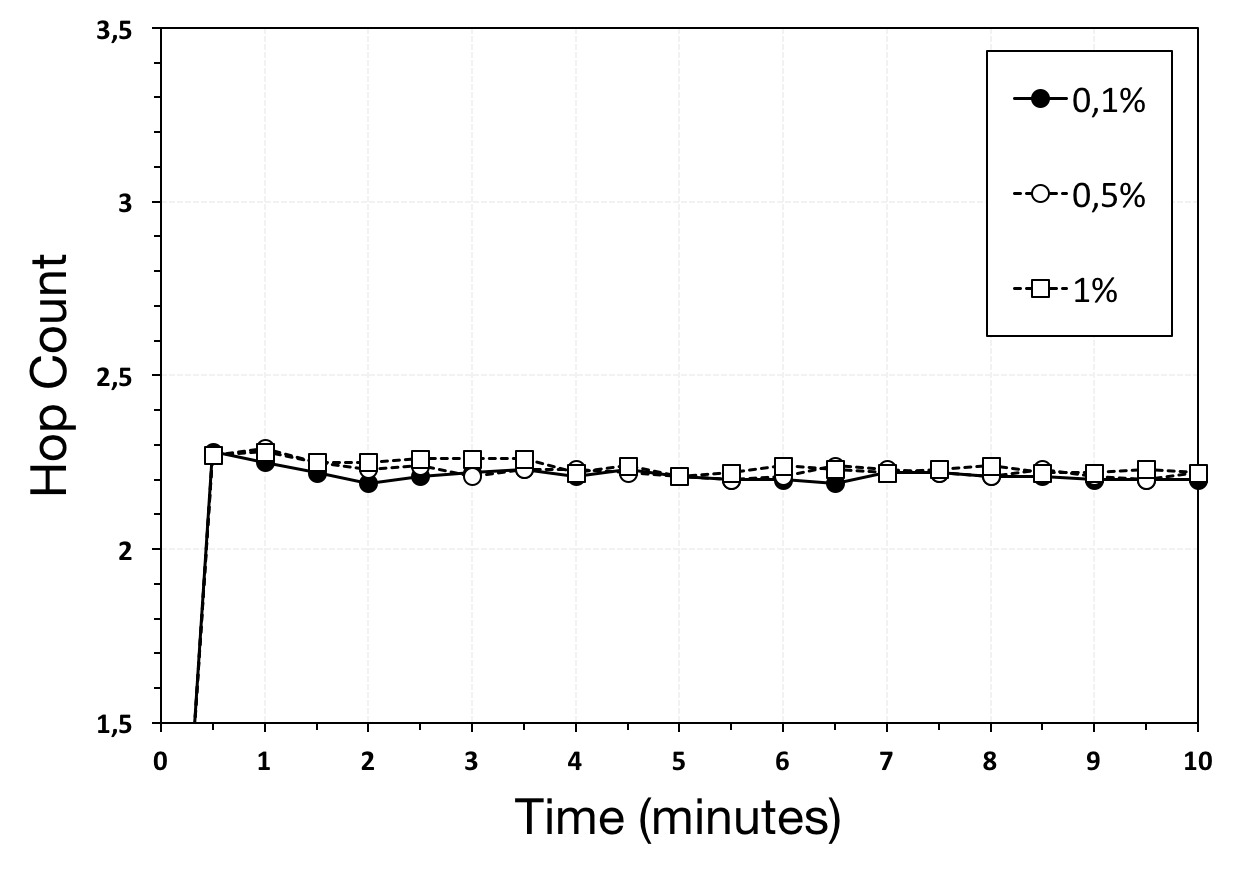
\includegraphics[keepaspectratio=true, width=1\linewidth]{images/average_hop_count_churn_1impl}
  \caption{}
  \label{fig:average_hop_count_churn_1impl}
\end{subfigure}%
\begin{subfigure}{.5\textwidth}
  \centering
  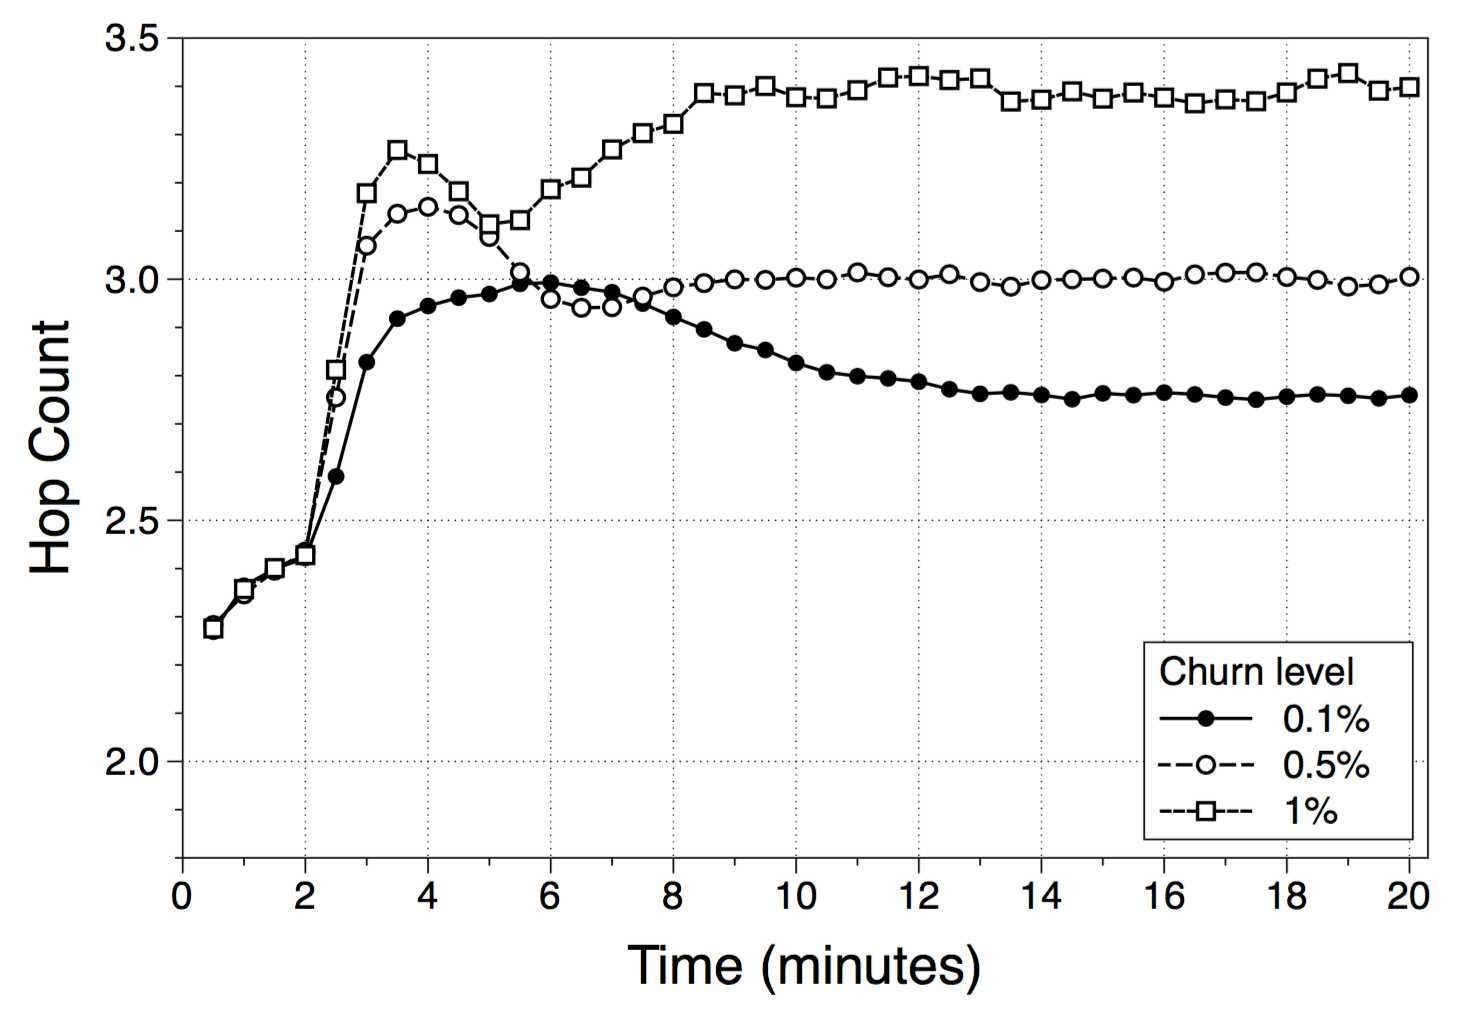
\includegraphics[keepaspectratio=true, width=1\linewidth]{images/paper_average_hop_count_churn}
  \caption{}
  \label{fig:paper_average_hop_count_churn}
\end{subfigure}
\caption{Average hop count under varying levels of churn. ~\ref{fig:average_hop_count_churn_1impl} represents our result,~\ref{fig:paper_average_hop_count_churn} is the test reported in the paper.}
\label{fig:robustness_hop_count_churn}
\end{figure}

\end{frame}

%-----------------------------------------------------------------------------------------------------------------------------
\section{Gossip-based aggregation protocol}

\begin{frame}[c]

\Huge{\centerline{Gossip-based aggregation protocol}}

\end{frame}


\begin{frame}
\frametitle{The idea}

Aggregation is a common name for a set of functions that provide a summary of some global system property. 

\begin{itemize}
  \item They allow local access to global information in order to simplify the task of controlling, monitoring and optimization in distributed applications
\end{itemize}

Examples of aggregation functions include network size, total free storage, maximum load, average uptime, etc.

\end{frame}

\begin{frame}
\frametitle{The idea}
\begin{itemize}
  \item The core of the protocol is a simple gossip-based communication scheme
  \item During this communication the nodes update their local approximate values
  \item All the approximate values in the system will quickly converge to the desired aggregate value
\end{itemize}
\end{frame}

\begin{frame}
\frametitle{Our case}
We consider the same network of the tests.
\begin{itemize}
  \item Each node in the network holds a numeric value
  \item We want to calculate the average among the nodes
\end{itemize}

In a practical setting, this value can characterize any aspect of the node or its environment (e.g., the load at the node, available storage space, temperature measured by a sensor network, etc.).

\end{frame}

\begin{frame}
\frametitle{First case}

\begin{itemize}
  \item All the nodes start with a random value between 0 and 1
  \item The expected output is the average over all these local values.
\end{itemize}
\end{frame}


\begin{frame}
\frametitle{First case result}
\begin{table}
\begin{tabular}{l l l}
\toprule
\textbf{Round} & \textbf{Minimum} & \textbf{Maximum}\\
\midrule
1 & 0.018574914802 & 0.996774217487 \\
2 & 0.070221341605 & 0.915147169418 \\
3 & 0.230152943376 & 0.833776234641 \\
4 & 0.289588175545 & 0.709077004544 \\
5 & 0.403064215889 & 0.597074271548 \\
6 & 0.450672692662 & 0.554978304631 \\
... & ... & ... \\
17  & 0.500661439413 & 0.500804356814 \\
18  & 0.500675542521 & 0.500750820268 \\
19  & 0.500703691477 & 0.5007381087 \\
20  & 0.500709860355 & 0.500727408936 \\
\bottomrule
\end{tabular}
\caption{Global average, minimum and maximum in each round.}
\end{table}
\end{frame}

\begin{frame}
\frametitle{First case}
    
\begin{figure}[p]
\centering
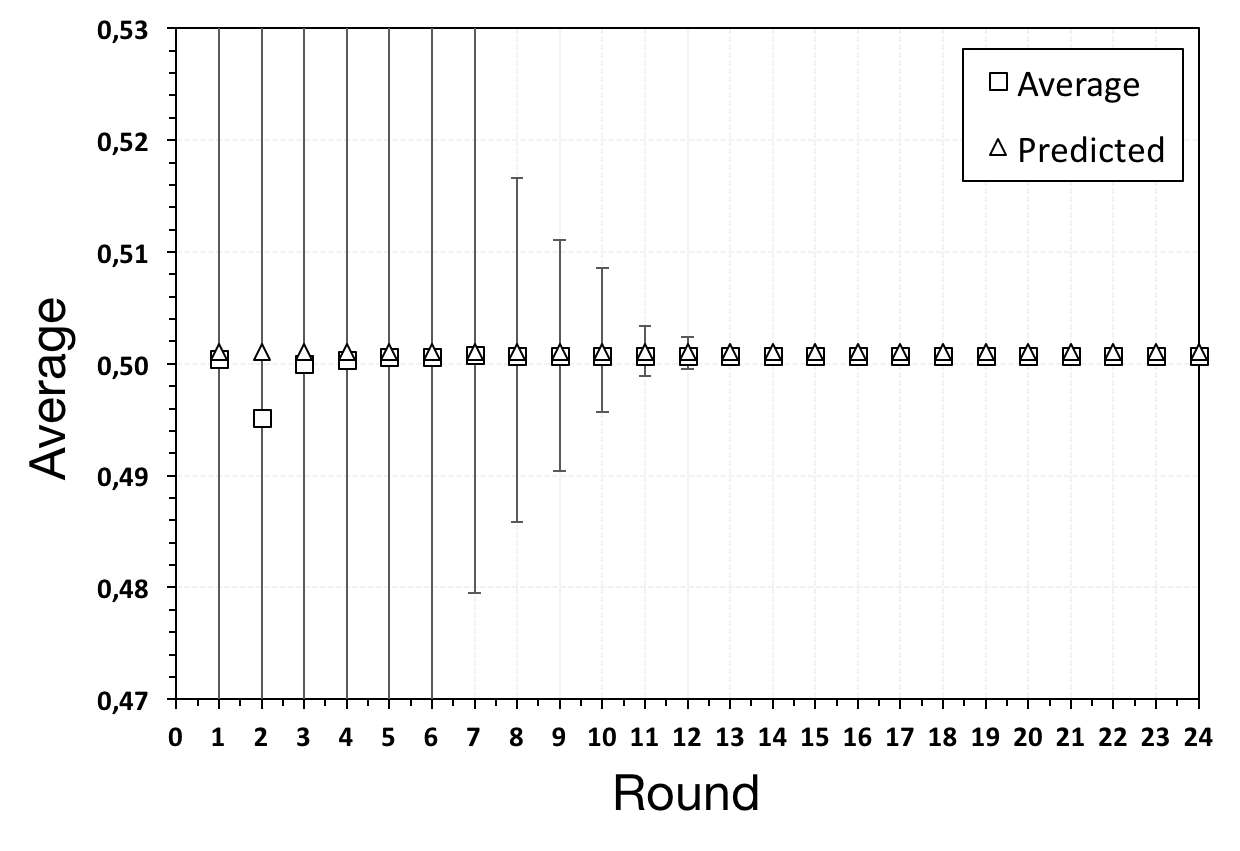
\includegraphics[keepaspectratio=true, width=0.8\linewidth]{images/aggregation_average}
\caption{Average evolution with error bars.}
\label{fig:aggregation_average}
\end{figure}
\end{frame}

\begin{frame}
\frametitle{First case}
    
\begin{figure}[p]
\centering
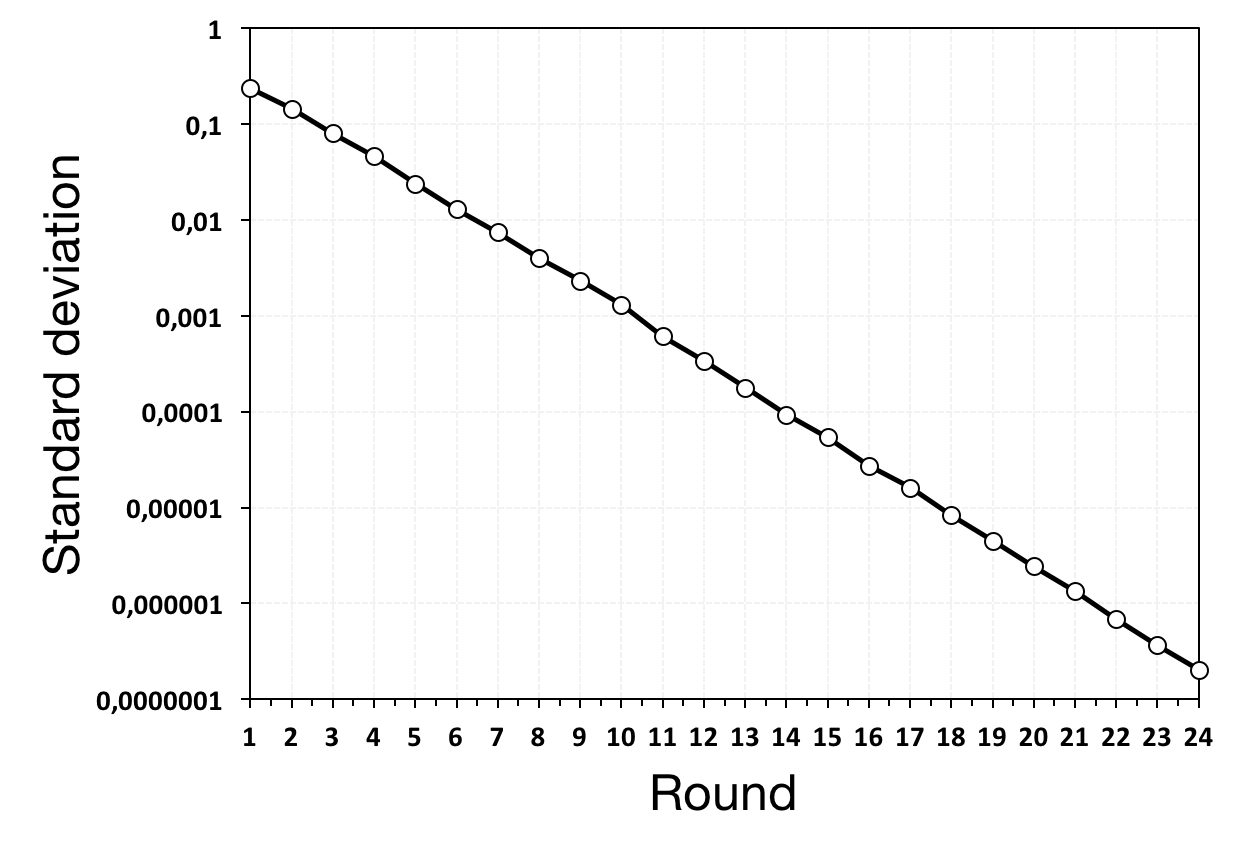
\includegraphics[keepaspectratio=true, width=0.8\textwidth]{images/aggregation_standard_deviation}
\caption{Standard deviation evolution.}
\label{fig:aggregation_standard_deviation}
\end{figure}

\end{frame}

\begin{frame}
\frametitle{Second case}

\begin{itemize}
  \item One node starts with 1 and the others with 0.
  \item The expected output is $1/N$, and if we do the inverse we obtain the total number of nodes present in the network (\textbf{Counting protocol}).
\end{itemize}
\end{frame}

\begin{frame}
\frametitle{Second case result}
\begin{table}
\begin{tabular}{l l}
\toprule
\textbf{Round} & \textbf{Average}\\
\midrule
1 & 0.0012617200674100 \\
2 & 0.0015042163745800 \\
3 & 0.0013683466120000 \\
4 & 0.0011746396263000 \\
5 & 0.0009807697464010 \\
6 & 0.0010497184912800 \\
... & ... \\
17  & 0.0010094031404220 \\
18  & 0.0010013031404250 \\
19  & 0.0010014001404220 \\
20  & 0.0010014031404250 \\
\bottomrule
\end{tabular}
\caption{Global average in each round.}
\end{table}
\end{frame}


\begin{frame}
\frametitle{Second case}

\begin{figure}[p]
\centering
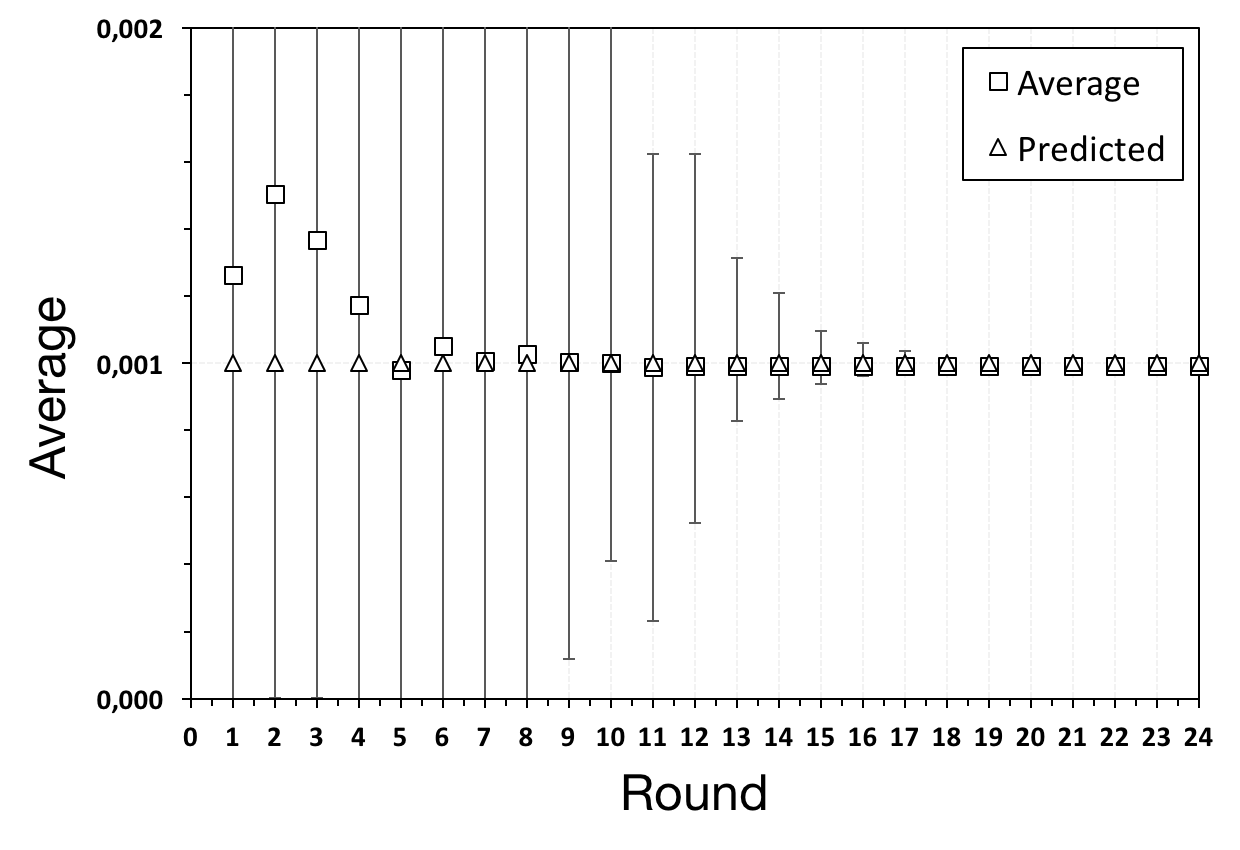
\includegraphics[keepaspectratio=true, width=0.8\textwidth]{images/counting_average}
\caption{Average evolution with error bars.}
\label{fig:counting_average}
\end{figure}

\end{frame}


\begin{frame}
\frametitle{Second case}
    
\begin{figure}[p]
\centering
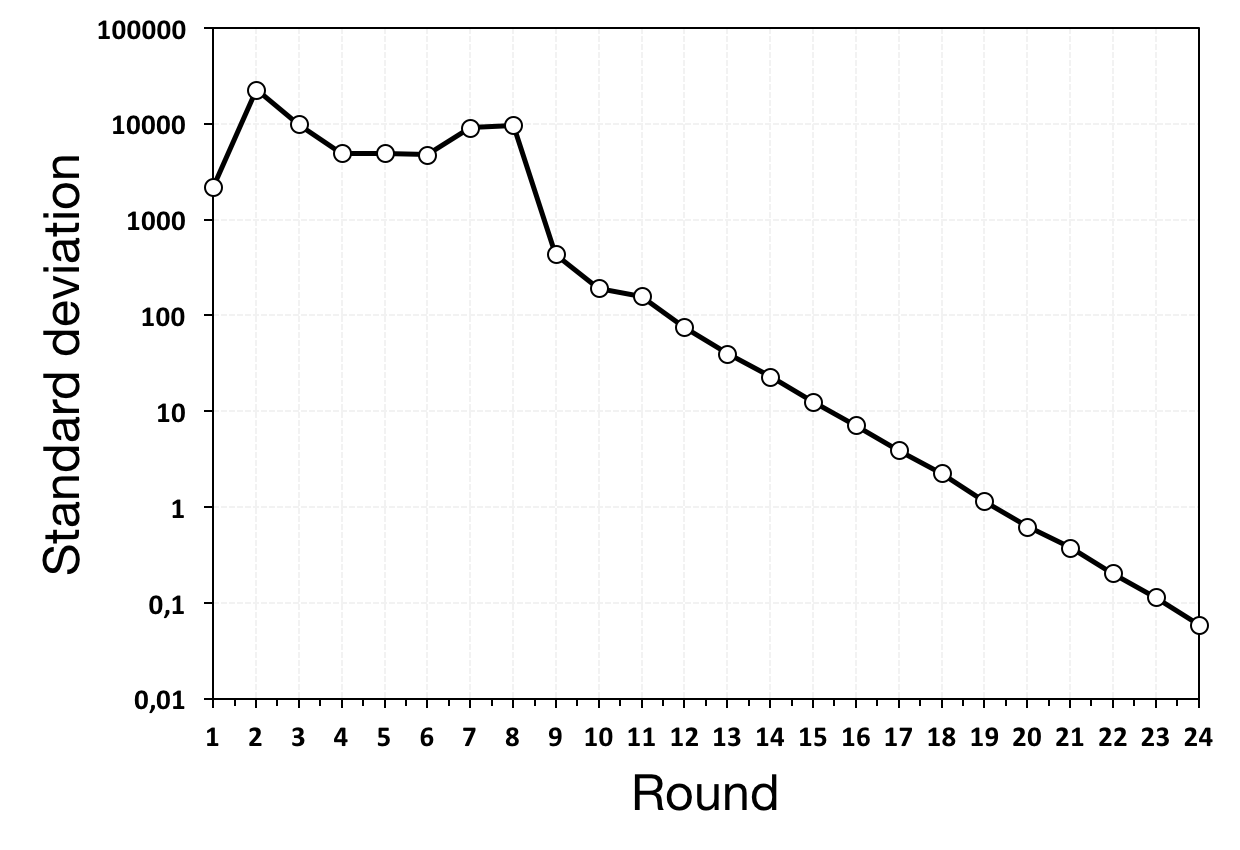
\includegraphics[keepaspectratio=true, width=0.8\textwidth]{images/counting_standard_deviation}
\caption{Standard deviation evolution.}
\label{fig:counting_standard_deviation}
\end{figure}

\end{frame}
%-----------------------------------------------------------------------------------------------------------------------------

\begin{frame}
\Huge{\centerline{The End}}
\end{frame}

%-----------------------------------------------------------------------------------------------------------------------------

\end{document} 